\section{Crescimento e Pontos de Extremo}
\begin{frame}
\frametitle{Funções Monótonas} 

\begin{definicao}\label{funcmon}
Seja $f: D \contido \R \to \R$ uma função. Dizemos que
\begin{enumerate}[(i)]
	\item $f$ é \sub{monótona (estritamente) crescente} se, para todos $x_1, x_2 \in D$,
	$$x_1 < x_2 \implica f(x_1) < f(x_2);$$
	\item $f$ é \sub{monótona não decrescente} se, para todos $x_1, x_2 \in D$,
	$$x_1 < x_2 \implica f(x_1) \leq f(x_2);$$
	\item $f$ é \sub{monótona (estritamente) decrescente} se, para todos $x_1, x_2 \in D$,
	$$x_1 < x_2 \implica f(x_1) > f(x_2);$$
	\item $f$ é \sub{monótona não crescente} se, para todos $x_1, x_2 \in D$,
	$$x_1 < x_2 \implica f(x_1) \geq f(x_2).$$%
%  \item $f$ é \sub{constante} se, para todo $x \in D$, temos $f(x) =
%  k \in \R$.
\end{enumerate}
\end{definicao}

\end{frame}



%------------------------------------------------------------------------------------------------------------
\begin{frame}
\frametitle{Funções Monótonas} 



Nas mesmas condições da Definição \ref{funcmon} , se $f(x) = k \in
\R$ para todo $x \in D$, dizemos que $f$ é \sub{constante}.\\ \pause
Se $I \contido D$ é um intervalo, definimos a monotonicidade de $f$
no intervalo $I$ de maneira análoga ao feito anteriormente. Por
exemplo: \\
$f$ é \sub{monótona (estritamente) crescente em $I$} se, para todos\\
$x_1, x_2 \in I$,
	$$x_1 < x_2 \implica f(x_1) < f(x_2).$$


\end{frame}



%------------------------------------------------------------------------------------------------------------

\begin{frame}
\frametitle{Funções Limitadas} 

\begin{definicao}
Seja $f: D \contido \R \to \R$ uma função.
\begin{enumerate}[(i)]
	\item $f$ é \sub{limitada superiormente} se existe $M \in \R$ tal
	que $f(x) \leq M$, para todo $x \in D$;
	\item $f$ é \sub{limitada inferiormente} se existe $M \in \R$ tal
	que $f(x) \geq M$, para todo $x \in D$;
	\item $x_0 \in D$ é um \sub{ponto de máximo absoluto} de $f$ se
	$f(x_0) \geq f(x)$, para todo $x \in D$;
	\item $x_0 \in D$ é um \sub{ponto de mínimo absoluto} de $f$ se
	$f(x_0) \leq f(x)$, para todo $x \in D$;
	\item $x_0 \in D$ é um \sub{ponto de máximo local} de $f$ se
	existe $r>0$ tal que $f(x_0) \geq f(x)$, para todo $x \in D \inter \paren{x_0 - r , x_0+r}$;
	\item $x_0 \in D$ é um \sub{ponto de mínimo local} de $f$ se
	existe $r>0$ tal que $f(x_0) \leq f(x)$, para todo $x \in D \inter \paren{x_0 - r ,
	x_0+r}$.
\end{enumerate}
\end{definicao}

\end{frame}



%------------------------------------------------------------------------------------------------------------


\begin{frame}
\frametitle{Exemplo} 
\begin{exemplo}
A função $h : \left( -1 ; 6 \right] \to \R$, cujo gráfico é esboçado
abaixo, é definida por $h(x) = \begin{cases}
																3x-x^2 & \ \text{ se } \ x\leq 2 \\
																\modu{x-4} +1 & \ \text{ se } \ 2 < x \leq 5 \\
																2 & \ \text{ se } \ x > 5 \\
																\end{cases}.$

\begin{center}
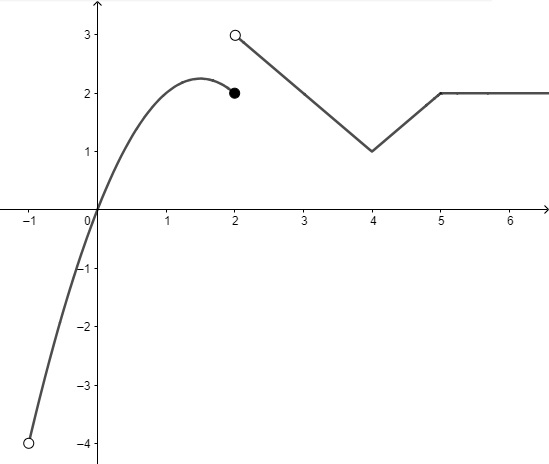
\includegraphics[width=3.8cm]{figures/funch.jpg}
\end{center}

Determine os intervalos de monotonicidade e os extremos de $h$.
\end{exemplo}
\end{frame}

%------------------------------------------------------------------------------------------------------------